\documentclass{article}

\usepackage[main=english,vietnamese]{babel}
\usepackage[T1]{fontenc}
\usepackage[utf8]{inputenc}
\usepackage[sexy]{evan}
\usepackage{matchsticks}
\usepackage{wrapfig}
\usepackage{listings}

\newtheorem{hint}{Hint}

\title{Solving Forty Two Problems by the Induction Principle - Part VII}
\author{Nghia Doan}
\date{\today}

\begin{document}

\maketitle

\begin{problem}[Problem Thirty Six]
    On the cirle of radius 1 with the center $O$ there are given $2n+1$ points $P_1P_2 \ldots P_{2n+1},$
    which lie on one side of a diameter. Prove that
    \[
        | \overrightarrow{OP_1} + \overrightarrow{OP_2} + \ldots  + \overrightarrow{OP_n} | \ge 1.
    \]
\end{problem}

\begin{soln}
    For $n=0$ we have $|\overrightarrow{OP_1} | = 1,$ thus the hypothesis stands.

    Assume that it is true for $2n+1$ vectors. By the Extremal Principle, there exists the maximal angle any two vectors,
    WLOG, let there be $\overrightarrow{OP_1}$ and $\overrightarrow{OP_{2n+3}}.$
    Now, by induction hypothesis,
    \[
        |\overrightarrow{OA}| = |\overrightarrow{OP_2} + \overrightarrow{OP_2} + \ldots  + \overrightarrow{OP_{2n+2}}| \ge 1 
    \]

    Note that $\overrightarrow{OA}$ is inside the angle $\angle P_1 O P_{2n+3},$ therefore it forms an acute angle with the vector 
    \[
        \overrightarrow{OB} = \overrightarrow{OP_1} + \overrightarrow{OP_{2n+3}}
    \]

    which bisects the angle $\angle P_1 O P_{2n+3}.$ Thus
    \[
        |\overrightarrow{OA} + \overrightarrow{OB}| \ge |\overrightarrow{OA}| = 1.
    \] 
\end{soln}

\begin{problem}[Problem Thirty Seven]
    $A_1 A_2 \ldots A_{2n}$ is a polygon inscribed in a circle. It is known that all the pairs of its opposite sides except one are parallel.
    Prove that for any odd $n$, the remaining pair of sides is also parallel.
    Prove that for $n$ even, the length of the exceptional sides are equal.
\end{problem}

\begin{center}
    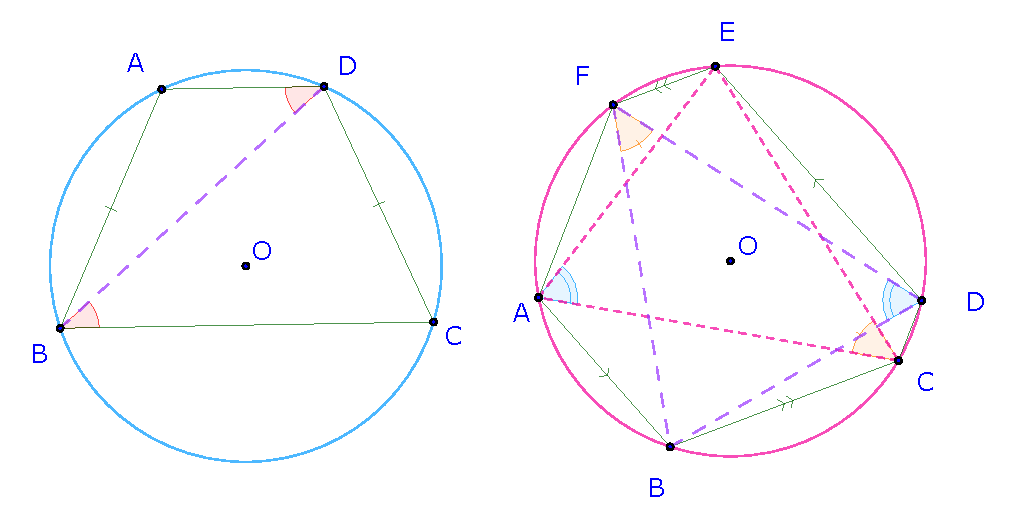
\includegraphics[width=8cm]{./svg/pdf/23-24-s5-o-p35.pdf}
\end{center}

\begin{soln}
    We first prove case $n=2$, note that in the left diagram $AD \parallel BC,$ then $\angle ADB = \angle CBD,$ thus $AB=CD.$

    For the case $n=3$, let $AB \parallel DE,$ so $\angle ACE = \angle BFD,$ and $ BC \parallel EF,$ so $\angle CAE = \angle BDF,$
    from here $\triangle CAE \sim \triangle FDB,$ or $\angle AEC = \angle DBF,$ thus $DC \parallel AF.$

    Let assume that the statement is true for $(2n-2)-$gon $A_1 A_2 \ldots A_{2n},$ where $A_1A_2 \parallel A_{n+1}A_{n+2},$ $\ldots,$
    $A_{n-1}A_n \parallel A_{2n-1}A_{2n}.$ Then considering the $(2n-2)-$gon $A_1A_2 \parallel A_{n-1}A_{n+1} \ldots A_{2n-1},$
    by the hypothesis, for $n$ odd: $A_{n-1}A_{n+1} = A_{2n+1}A_1$ and for $n$ even $A_{n-1}A_{n+1} \parallel A_{2n-1}A_1.$

    Consider now the triangles $A_{n-1}A_nA_{n+1}$ and $A_{2n-1}A_{2n}A_1.$
    
    \textit{Case 1:} if $n$ is even. then $\overrightarrow{A_{n-1}A_n}$ and $\overrightarrow{A_{2n-1}A_{2n}}$ as well as 
    $\overrightarrow{A_{n-1}A_{n+1}}$ and $\overrightarrow{A_{2n-1}A_{2n}}$ are parallel and oppositely directed.
    Hence $\angle A_nA_{n-1}A_{n+1} = \angle A_1 A_{2n-1} A_{2n}$ and $A_nA_{n+1} = A_{2n}A_1$ since they are chords that cut equal arcs.

    \textit{Case 2:} if $n$ is odd. then $A_{n-1}A_{n+1} = A_{2n-1}A_2,$ i.e. $A_1 A_{n-1} \parallel A_{n+1}A_{2n-1}.$ 
    In the hexagon $A_{n-1}A_n A_{n+1}A_{2n-1}A_{2n}A_{1}$ we have $A_1 A_{n-1} \parallel A_{n+1}A_{2n-1},$ $A_{n-1}A_n \parallel A_{2n-1}A_{2n},$
    hence from the base case $n=3,$ $A_nA_{n+1} \parallel A_{2n-1}A_1.$ 
\end{soln}

\begin{problem}[Problem Thirty Eight]
    Let 
    \[ 
        a_1 = a_2 = 1,\ a_{n+2} = a_{n+1} + \frac{a_n}{3^n},\ \forall n \ge 1.
    \]

    Prove that $a_n \le 2,\ \forall n \ge 1.$
\end{problem}

\begin{soln}
    Let's prove that $a_n \le 2 - \frac{1}{3^{n-2}},\ \forall n \ge 2 \quad (*)$
    
    For $n=2$, $a_2 = 1 \le 2 - \frac{1}{3^{0}} = 1.$ For $n=3,$ $a_3 = a_2 + \frac{a_1}{3^1} = 1 + \frac{1}{3} < 2 - \frac{1}{3}.$

    Let's assume that (*) stand for all $k \le n,$ $n\ge 3,$ then
    \[
        a_{n+1} = a_{n} + \frac{a_{n-1}}{3^{n-1}} < 2 - \frac{1}{3^{n-2}} + \frac{2}{3^{n-1}} - \frac{1}{3^{2n-4}}
        = 2 - \frac{1}{3^{n-1}} - \frac{1}{3^{2n-4}} < 2 - \frac{1}{3^{n-1}}.
    \]
\end{soln}

\begin{problem}[Problem Thirty Nine]
    Let $x_0, x_1, \ldots, x_{1995}$ be positive real numbers,
    \[ 
        x_0 = x_{1995} = 1,\ x_{n-1} +\frac{2}{x_{n-1}} = 2x_n + \frac{1}{x_n}, \ \forall n=1,2,\ldots,1995
    \]

    Find the maximal value that $x_0$ can have.
\end{problem}

\begin{soln}
    First 
    \[
        x_{n-1} +\frac{2}{x_{n-1}} = 2x_n + \frac{1}{x_n} \Leftrightarrow (2x_n - x_{n-1})(x_{n} x_{n-1} -1) = 0
        \Rightarrow x_n = \frac{1}{2} x_{n-1}, \text{\ or\ } x_n = \frac{1}{x_{n-1}}.
    \]

    We prove by induction that 
    \[
        x_n = 2^{k_n}x_0^{e_n},\ k_n \in \ZZ,\ |k_n| \le n,\ e_n = (-1)^{n-k_n}.
    \]

    This is true for $n=0.$ Assume that it is true for some $n,$ then
    \[
        \begin{aligned}
            &x_{n+1} = \half x_n = 2^{k_n-1}x_0^{e_n} = 2^{k_{n+1}} x_0^{e_{n+1}},\
            \text{where}\ k_{n+1} = k_n-1, e_{n+1} = (-1)^{n-k_n} = (-1)^{(n+1)-(k_n-1)},\\
            &x_{n+1} = \frac{1}{x_n} = 2^{-k_n} x_0^{-e_n} = 2^{k_{n+1}} x_0^{e_{n+1}}
            \ \text{where}\ k_{n+1} = -k_n, e_{n+1} = (-1)^{n-k_n+1} = (-1)^{(n+1)-(k_n)}.\\
        \end{aligned}
    \]

    Now $x_ 0 = x_{1995} = 2^{k_{1995}} x_0^{e_{1995}},$ so, $e_{1995} = (-1)^{1995 - k_{1995}}.$
    $e_{1995}$ cannot be $1$ because then $k_{1995}$ would be odd, contradicting that $2^{k_{1995}} = 1.$
    So $e_{1995} = -1,$ thus $x_0^2 = 2^{k_{1995}} \le 2^{1994}.$

    Thus the maximal value of $x_0$ is $\boxed{2^{997}.}$
     
    When this can happen? $x_k = 2^{997-k}$ for $k=0,1,\ldots, 1994,$ and $x_{1995} = (x_{1994})^{-1} = 2^{997}.$
\end{soln}

\begin{problem}[Problem Fourty]
    Let $a_0 > 5$ be an odd integer,
    \[ 
        a_{n+1} = 
        \begin{cases}
            &a_n^2 - 5 \text{\ if\ } a_n \text{\ is odd},\\
            &\half a_n \text{\ otherwise}
        \end{cases}
        \ \forall n\ge 0
    \]

    Prove that this sequence is not bounded.
\end{problem}

\begin{soln}
    We prove that 
    \begin{claim*}
        $a_{3n}$ is odd, $a_{3n} > a_{3n-3} > \ldots > a_0 > 5.$
    \end{claim*}
    \begin{subproof}
        It is easy to verify the case $a_0 > 5,$ odd integer.
        Let assume $a_{3n}$ is odd, so $a_{3n + 1} = a_{3n}^2 - 5 \equiv 4 \Mod{8}.$
        This means that $a_{3n+2} = \half a_{3n + 1},$ $a_{3n + 3} = \half a_{3n + 2},$ and
        $a_{3n + 3}$ is odd.

        In addition $a_{3n + 3} \frac{1}{4} (a_{3n}^2 - 5) > a_{3n},$ ($a_{3n} > 5$)
        thus $a_{3n + 3} > a_{3n}.$
    \end{subproof}
\end{soln}

\begin{problem}[Problem Fourty One]
    Let $x$ be a real number and $n \ge 1$ positive integer. Prove that
    \[ 
        | \sin {(nx)} | \le n |\sin{x}|.
    \]
\end{problem}

\begin{soln}
    The case $n=1$ is clear.

    For the inductive step, consider
    \[
        |\sin(n+1)x = |\sin(nx)\cos(x) + \cos(nx)\sin(x)| \le |\sin(nx)| + |\sin(x)|.
    \]
\end{soln}

\begin{problem}[Problem Fourty Two]
    Prove that for $a > 0$ and $n$ positive integer:
    \[ 
        2(1 + a^{n+1})^3 \ge (1+a^3) (1+a^n)^3
    \]

    Prove that for $a,b,c$ positive real numbers,
    \[
        2(a^{2023} + 1)(b^{2023} + 1)(c^{2023} + 1) \ge (1+abc)(a^{2022} + 1)(b^{2022} + 1)(c^{2022} + 1).
    \]
\end{problem}

\begin{soln}
    For $a > 0$ and $n$ positive integer, we prove by induction that:
    \begin{claim*}
        $2(1 + a^{n+1})^3 \ge (1+a^3) (1+a^n)^3.$
    \end{claim*}
    \begin{subproof}
        For $n=1$ then 
        \[
            2(1+a^2)^3 \ge (1+a^3) (1+a)^3 \Leftrightarrow (a-1)^4 (a^2+a+1)
        \]
    
        Assume that it is true for $n$, or
        \[
            2(1+a^{n+1})^3 \ge (1+a^3) (1+a^{n})^3.
        \]
    
        Since
        \[
            \begin{aligned}
                &(1 + a^{n+2})(1+a^n) \ge (1+a^{n+1})^2 \Rightarrow \frac{1+a^{n+2} }{1+a^{n+1}} \ge \frac{1+a^{n+1}}{1+a^n}\\
                &\Rightarrow 2(1+a^{n+2})^3 = 2 (1+a^{n+1})^3 \left( \frac{ 1+a^{n+2}}{1+a^{n+1}}\right)^3\\
                &\ge (1+a^3) (1+a^{n})^3 \left( \frac{ 1+a^{n+1}}{1+a^{n}}\right)^3
                = (1+a^3) (1+a^{n+1})^3
            \end{aligned}
        \]
    \end{subproof}

    Now it is easy to verify that
    \[
        (1+a^3)(1+b^3(1+c^3) \ge (1+abc)^3.
    \]

    Then 
    \[
        \begin{aligned}
            &(2(a^{2023} + 1)(b^{2023} + 1)(c^{2023} + 1))^3 = 2 (a^{2023} + 1)^3 \cdot 2 (b^{2023} + 1)^3 \cdot 2 (c^{2023} + 1)^3 \\
            &\ge (1+a^3)(1+a^{2022} + 1)^3 \cdot (1+b^3)(1+b^{2022} + 1)^3 \cdot (1+c^3)(1+c^{2022} + 1)^3\\
            &\ge (1+abc)^3 ((a^{2022} + 1)(b^{2022} + 1)(c^{2022} + 1))^3
        \end{aligned}
    \]

    By taking cubic root, the result follows.
\end{soln}

\end{document}